\subsection{Opgave 23}

En vektor $\Vec{c}$ har længden 6 og retningsvinklen $127^{\circ}$\\\\
Bestem koordinaterne for $\Vec{c}$.\\\\

\ans
For at bestemme vektor c's koordinaterne gør vi bruge af følgende formel
\begin{align*}
    \Vec{c} = \begin{pmatrix}l\cdot \cos(v) \\ l\cdot \sin(v)\end{pmatrix}
\end{align*}
Her er l vektorens længde og v er vektorens retningsvinkel. Indsætter vi de givne værdier får vi
\begin{align*}
    \Vec{c} = \begin{pmatrix}6\cdot \cos(127^{\circ}) \\ 6\cdot \sin(127^{\circ})\end{pmatrix} = \begin{pmatrix}-3.61 \\ 4.79\end{pmatrix}
\end{align*}
Vektoren er illustreret nedenfor\\\\
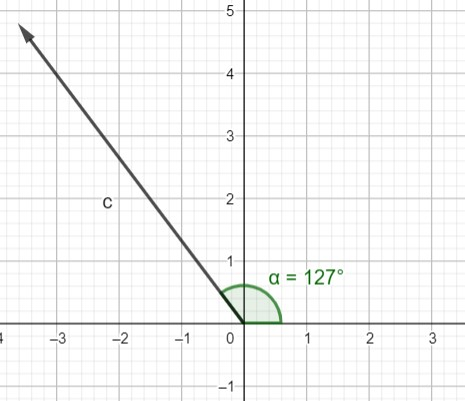
\includegraphics[width = 6cm]{Opgave_21-30/Opgave_23/23.jpg}